\documentclass{standalone}
\usepackage{tikz}
\begin{document}

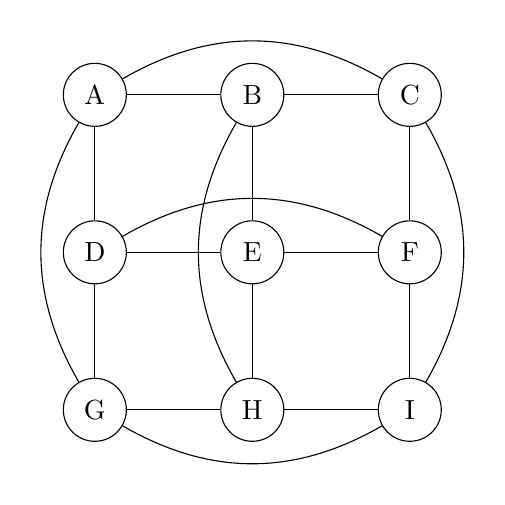
\begin{tikzpicture}[every node/.style={circle, draw, minimum size=8mm}]

% Rook's Graph R_3,3

\node (A) at (0,0) {A};
\node (B) at (2,0) {B};
\node (C) at (4,0) {C};
\node (D) at (0,-2) {D};
\node (E) at (2,-2) {E};
\node (F) at (4,-2) {F};
\node (G) at (0,-4) {G};
\node (H) at (2,-4) {H};
\node (I) at (4,-4) {I};

\foreach \from/\to in {A/B, A/D, B/E, C/F, B/C,
                       D/E, D/G, E/H, F/I,
                       G/H, H/I, E/F}
    \draw (\from) -- (\to);

\draw [bend left] (A) to (C);
\draw [bend left] (D) to (F);
\draw [bend right] (G) to (I);
\draw [bend right] (A) to (G);
\draw [bend right] (B) to (H);
\draw [bend left] (C) to (I);

\end{tikzpicture}

\end{document}